\chapter{PROJEKT SYSTEMU}

tekst, tu już typowo o naszej implementacji (porównywać do papieru), na początku krótki opis że dzieli sie na front i backend i model


\section{Interfejs gry \textit{Kacper Konopka}}

% cały opis unity, za co odpowiada, jakie są interakcje, animacje
Aby przedstawić świat, w którym operują agenci stworzone zostały interfejsy ułatwiające interpretacje przez człowieka. Dzięki nim osoba uczestnicząca jest w stanie zaobserwować zachowania agentów jako grę. Do stworzenia takiego środowiska użyto silnik do gier Unity, który zawiera wiele elementów interaktywnych pozwalających zarówno tworzyć agentów jak i zobaczyć ich aktualny stan. Oprócz części, w których obserwator może wpływać na środowisko są również te, które prezentują elementy otoczenia np. drzewa, domy bądź rzeki.

\subsection{Elementy interaktywne}
Celem stworzenia imersji obserwator ma możliwość ingerowania w świat agentów poprzez następujące elementy.
\subsubsection{Interfejs tworzenia nowych agentów}
W ramach udostęnienia możliwości tworzenia nowych agentów stworzono okno, w którym użytkownik wprowadza informacje na temat agenta. Każde z pól - imię (ang. \textit{Name}), wiek (ang. \textit{Age}), opis agenta (ang. \textit{Description}) oraz styl życia (ang. \textit{Lifestyle}) musi zostać wypełnione aby agenta stworzyć. W przeciwnym przypadku przy naciśnięciu przycisku \textit{Submit} gra poinformuje nas o tym, że jedno z tych pól jest puste a agent nie zostanie stworzony. Oprócz wypełnienia informacji tekstowych możemy również wybrać wygląd agenta spośród uprzednio stworzonych zasobów. Gdy użytkownik nie wybierze modelu postaci, dobierany jest pierwszy zasób z listy. Aby zakończyć tworzenie agenta użytkownik musi nacisnąć przycisk \textit{Submit}. Gdy wszystkie wyżej wymienione warunki są spełnione agent pojawia się na środku mapy.
Wypełniony interfejs prezentuje rysunek~\ref{fig:createagent}.
\begin{figure}[htbp]
    \centering
    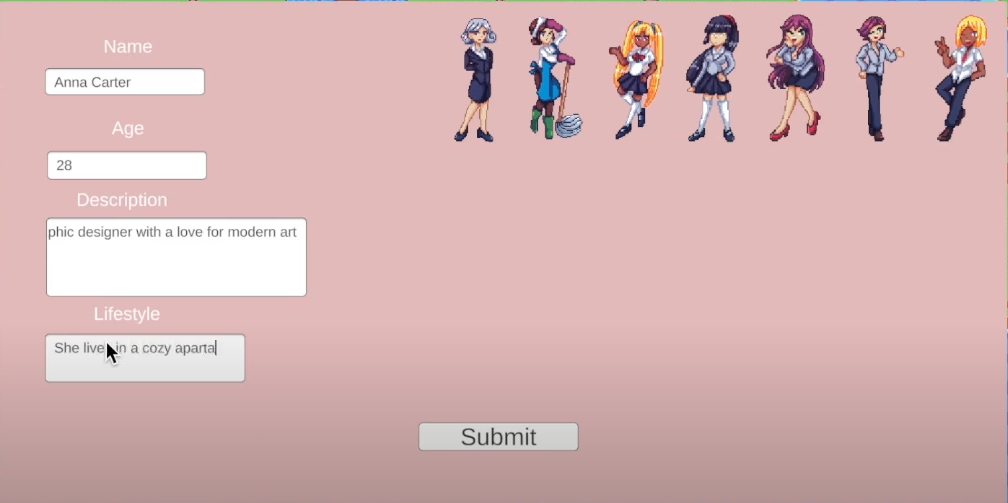
\includegraphics[width=0.9\textwidth]{images/411.png}
    \caption{Rysunek przedstawiający przykładowy, prawidłowo wypełniony interfejs tworzenia agenta.}
    \label{fig:createagent}
\end{figure}
\subsubsection{Interfejs stanu agenta}
Ważnym elementem obserwacji działania agentów jest wyświetlanie ich stanu. W tym celu stworzono interfejs, który wyświetla podstawowe informacje o agencie. Aby uzyskać informacje o agencie należy kliknąć na agenta, który znajduje się w polu widzenia. W skład danych, które znajdują się w oknie znajdują się elementy takie jak - aktualna data i godzina wydarzeń, identyfikator agenta, imię (ang. \textit{Name}), wiek (ang. \textit{Age}), opis agenta (ang. \textit{Description}) oraz styl życia (ang. \textit{Lifestyle}). Przrykładowy stan agenta ukazany jest w rysunku~\ref{fig:stateagent}. Okno interfejsu stanu agenta jest półprzezroczyste, przez co można zauważyć niektóre elementy środowiska, które nie przeszkadzają w interpretacji przedstawionych danych.
\begin{figure}[htbp]
    \centering
    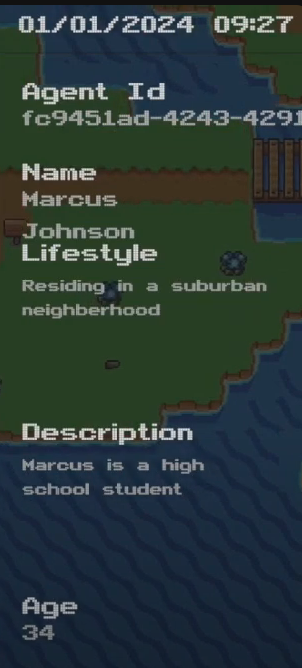
\includegraphics[width=0.9\textwidth, height=0.6\textheight]{images/411state.png}
    \caption{Rysunek przedstawiający przykładowy interfejs stanu agenta.}
    \label{fig:stateagent}
\end{figure}


\section{Architektura serwera i warstwy logicznej}
\label{sec:architektura_serwera}

\subsection{Agenci}

\subsubsection{Pamięć agentów}
Pamięć agentów jest kluczowym elementem ich funkcjonowania.
To dzięki niej agenci reagują w sposób bardziej ludzki.

\paragraph{Architektura pamięci agentów}
Pamięć opiera się na modelu języka naturalnego typu encoder, który przekształca
nowe wspomnienia agenta na wektor. Później, w trakcie interakcji czy budowania nowych
wspomnień przez agenta jest wybierane k wspomnień, które uzyskały największą średnią
ważoną z trzech metryk: podobieństwa (relevance), ważności (importance) i niedawności (recency).
Wybrane wspomnienia są później przekazywane do modelu językowego typu decoder, który na
podstawie ich i danego wydarzenia decyduje o zachowaniu agenta.

\paragraph{Metryka podobieństwa}
Metryka podobieństwa odpowiada podobieństwu tematycznemu nowego wydarzenia do
wydarzenia zapisanego w pamięci agenta. Jest to uzyskiwane za pomocą obliczonej
odległości cosinusowej wektorów stworzonych przez model typu encoder.

\paragraph{Metryka ważności}
Metryka istoty jest uzyskiwana
poprzez ocenę ważności danego wydarzenia w kontekście życia agenta przez LLM.
Metryka odpowiada na pytanie jak ważne dla danego agenta w skali od 1 do 10 jest
dane wydarzenie np. pościelenie łóżka będzie miało skalę bliską 1, gdzie wzięcie
ślubu skalę bliską 10.

\paragraph{Metryka niedawności}
Metryka niedawności odpowiada mechanizmowi "zapominania" przez agenta.
Wspomnienia uzyskują wynik zgodnie ze wzorem:

\begin{equation}
 \label{eq:metryka_niedawnosci}
	score = max\_score * decay\_factor ^ {time\_diff}
\end{equation}




\section{Polecenia dla modeli językowych}

% przenieść do teorii 
Jakość odpowiedzi generowanych przez duże modele językowe w znacznym stopniu zależy od~zapytań, które są do nich wysyłane. Tekst przekazywany do modelu nazywany jest poleceniem (ang. \textit{prompt}), którego główną częścią jest pytanie lub zadanie opisujące, co model powinien wykonać. W przypadku techniki RAG w skład polecenia wchodzi także kontekst, czyli tekst ukazujący szerszą perspektywę danego tematu. W~samym zadaniu zawarta jest także informacja dla modelu, aby ten, podczas odpowiadania na pytanie lub wykonywania postawionego mu zadania, korzystał bezpośrednio z dostarczonego mu kontekstu - jeżeli jakaś informacja w nim nie występuje, model powinien jasno zakomunikować, że nie jest w stanie odpowiedzieć na pytanie. Nie powinien próbować wymyślać odpowiedzi jedynie na podstawie własnej wiedzy.

\subsection{Wykonywanie akcji}

W aplikacji SMIS, podobnie jak w programie, na którym wzorowana jest jej implementacja~\cite{park2023generativeagentsinteractivesimulacra}, każda decyzja dotycząca przebiegu rozgrywki podejmowana jest za pomocą dużego modelu językowego. W~ujęciu ogólnym, na podstawie otrzymanych odpowiedzi, wykonywane są odpowiednie akcje. Kiedy rozpoczyna się dzień, dla każdego agenta generowany jest godzinowy plan dnia, bazujący na~jego zainteresowaniach i jego trybie życia. Agent przeżywa dzień zgodnie z tym planem. Ponadto, przy~każdym spotkaniu z inną osobą, model językowy decyduje, czy agenci powinni nawiązać konwersację. Jeśli decyzja jest pozytywna, tworzona jest konwersacja, która nawiązuje do~wspomnień rozmówców oraz jest zgodna z~ich osobowościami. Po zakończeniu rozmowy jest ona podsumowywana i generowane są wspomnienia dla obu agentów, które zapisywane są w~ich pamięci. Dzięki temu mogą się oni do nich odwoływać w odpowiednich do tego momentach.

Przy tworzeniu polecenia dla modelu, pobierane są informacje i wspomnienia odnoszące się do~konkretnego agenta. Żeby proces ten mógł nastąpić, należy podczas zapisywania wspomnienia uwzględnić trzy metryki, opisane szerzej w podrozdziale \ref{sec:architektura_serwera}. Metryka ważności również opiera się na odpowiedzi od modelu.

\subsection{Konwersacje}

Tworzenie konwersacji jest dość skomplikowanym procesem. Aby jak najbardziej upodobnić agentów do prawdziwych ludzi, generowanie rozmowy podzielone zostało na kilka etapów.

Pierwszym z nich jest decydowanie, czy agent powinien w ogóle podjąć konwersację. Warto zauważyć, że my również nie odzywamy się do każdej miniętej na ulicy osoby - w takiej sytuacji nie udawałoby nam się nigdzie dotrzeć, gdyż cały dzień wypełniony byłby jedynie rozmowami z innymi. Podświadomie oceniamy, czy warto przywitać się z daną osobą. Czynniki, jakie są w takiej sytuacji brane pod uwagę, to m.in. to, kim jest spotkany człowiek, czy go znamy, co w danym momencie robi, czy nie jest zajęty.

Podobnie działają agenci w aplikacji SMIS.




\section{Komunikacja między serwisami}

jak jest zrobiona komunikacja, jak to działa, może być wiele frontów na jeden serwer
